Nous avons choisi un ensemble d'opération que nous avons alors détaillé
et analyser afin de s'assurer de leur correct fondement, de leur cohérence
avec les autres modèles et de la correcte controlabilité/monitoribilité
des agents qui doivent procéder à ces opérations.

\subsection{RecordAmbulanceAvailability}

Avant tout chose, il est nécessaire de situer l'opération dans le modèle
des buts. La figure \ref{fig:tab:RecordAmbulanceAvailability:goal} montre
où est situé le but correspondant à l'opération ainsi que l'agent responsable
de la bonne réalisation de ce but.
\begin{figure}[!h]
	\begin{center}
		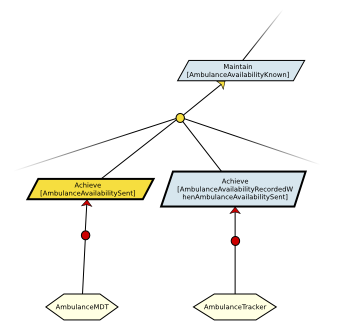
\includegraphics[scale=1]{images/RecordAmbulanceAvailabilitGoal.png}
		\caption{Le but attaché à l'opération RecordAmbulanceAvailability.}\label{fig:tab:RecordAmbulanceAvailability:goal}
	\end{center}
\end{figure}

Nous pouvons donc synthétiser ces informations dans le tableau \ref{tab:RecordAmbulanceAvailability:goalandagent}
\begin{table}
	\begin{tabular}{|l|l|}\hline
	But correspondant & Achieve[AmbulanceAvailabiltyRecordedWhenAmbulanceAvailabilitySent] \\ \hline
	Agent & AmbulanceTracker
	\end{tabular}
	\caption{Récapitulatif du but opérationnalisé et de l'agent qui va procéder à cette opération.}\label{tab:RecordAmbulanceAvailability:goalandagent}
\end{table}

Les objets nécessaires à la réalisation de cette opération sont \textit{AmbulanceInfo}
et \textit{AvailabilityMessage}.

\begin{table}
	\begin{tabular}{|l|l|}\hline
In:  	&avlbM: AvailabilityMessage, AmbulanceInfo\\ \hline
Pre: 	&Exists amb: AmbulanceInfo : amb.ambulanceName = avlbM.ambulanceName\\ \hline

Out:  	&amb: AmbulanceInfo\\ \hline
Post:	&mdtM.availability = true $<=>$ amb.infoMobilization is not null \\ \hline
	&mdtM.availability = false $<=>$ amb.infoMobilitzation is null\\ \hline
	\end{tabular}
	\caption{fff}
\end{table}
